
%%%%%%%%%%%%%%%%%%%%%%% file typeinst.tex %%%%%%%%%%%%%%%%%%%%%%%%%
%
% This is the LaTeX source for the instructions to authors using
% the LaTeX document class 'llncs.cls' for contributions to
% the Lecture Notes in Computer Sciences series.
% http://www.springer.com/lncs       Springer Heidelberg 2006/05/04
%
% It may be used as a template for your own input - copy it
% to a new file with a new name and use it as the basis
% for your article.
%
% NB: the document class 'llncs' has its own and detailed documentation, see
% ftp://ftp.springer.de/data/pubftp/pub/tex/latex/llncs/latex2e/llncsdoc.pdf
%
%%%%%%%%%%%%%%%%%%%%%%%%%%%%%%%%%%%%%%%%%%%%%%%%%%%%%%%%%%%%%%%%%%%


\documentclass[runningheads,a4paper]{llncs}

\usepackage{amssymb}
\setcounter{tocdepth}{3}
\usepackage{graphicx}

\usepackage{url}
\urldef{\mailsa}\path|{alfred.hofmann, ursula.barth, ingrid.haas, frank.holzwarth,|
\urldef{\mailsb}\path|anna.kramer, leonie.kunz, christine.reiss, nicole.sator,|
\urldef{\mailsc}\path|erika.siebert-cole, peter.strasser, lncs}@springer.com|    
\newcommand{\keywords}[1]{\par\addvspace\baselineskip
\noindent\keywordname\enspace\ignorespaces#1}

\usepackage{nameref}
\begin{document}

\mainmatter  % start of an individual contribution

% first the title is needed
\title{DAT530\\Discrete Simulation and Performance Analysis\\Final Project\\Solitaire game strategy}

% a short form should be given in case it is too long for the running head
\titlerunning{DAT530 - Final Project}

% the name(s) of the author(s) follow(s) next
%
% NB: Chinese authors should write their first names(s) in front of
% their surnames. This ensures that the names appear correctly in
% the running heads and the author index.
%
\author{Racin W. Nygaard}%

%
\authorrunning{DAT530 - Final Project - Solitaire game strategy}
% (feature abused for this document to repeat the title also on left hand pages)

% the affiliations are given next; don't give your e-mail address
% unless you accept that it will be published
\institute{Universitetet i Stavanger}

%
% NB: a more complex sample for affiliations and the mapping to the
% corresponding authors can be found in the file "llncs.dem"
% (search for the string "\mainmatter" where a contribution starts).
% "llncs.dem" accompanies the document class "llncs.cls".
%

\toctitle{Solitaire game strategy}
\tocauthor{Report}
\maketitle


\begin{abstract}
SKRIV DETTE TIL SLUTT!
This document describes how we were able to extract relevant information from the Enron Email Dataset using 7 different MapReduce jobs. All of our code in the jobs was written in Python, source code can be found in our git repository \cite{git}. Where applicable we have attempted to visually present our results.
\newline
The dataset provided contained a large amount of duplicate email, and to improve the results of some selected jobs, we adjusted our algorithms to remove them.
\newline
By extracting the same information in MapReduce and Hive we were able to compare running times of the two for one particular task.
\end{abstract}


\section{Introduction}
The objective of the project was to locate relevant information in a dataset of emails using Hadoop. It was up to the group to create a set of tasks, and to extract the required information from the dataset in order to complete them.
\newline
\newline
In total, we have created 7 tasks of different complexity. Detailed explanation about each task can be found in the subsections of section~\ref{sec:mapreducealgorithms}.
\newline
The first task, \texttt{\nameref{sec:41_counting}}, was created to gain better insight into the dataset. This insight provided us with the possibility to exclude duplicate messages, and filter out invalid messages. This is discussed further in section~\ref{sec:2_dataset}.
\newline
In the second task, \texttt{\nameref{sec:emailthreads}} we wanted to determine how long an email thread lasted, and how many participants were involved. For the third task, \texttt{\nameref{sec:sendtimes}}, the information we wanted to extract was how many emails the employees of Enron sent at different times during a full week.
\newline
For the fourth task, \texttt{\nameref{sec:comstruct}}, we wanted to split the employees of Enron into clusters, grouping the ones who communicate more with each other, than the rest of the organisation.
\newline
The fifth task, \texttt{\nameref{sec:tfids}}, provides the possibility to search for specific words and phrases in the email set. In addition it will score the results after how important the word or phrase is in the email. The sixth task, \texttt{\nameref{sec:topsender}}, ranks each email-sender by how many emails they have sent. The final output is sorted in descending order, and thereby provides an efficient source for fetching the top X senders.
\newline
The last task we created was \texttt{\nameref{sec:bkmeans}}. Here we have implemented bisecting K-means clustering in a 7-step MapReduce job.
\newline
\newline
In addition to these tasks, the dataset is discussed in detail in section~\ref{sec:2_dataset}. In section~\ref{sec:hadoop} we provide some insight on how we set up Hadoop for this project. Then follows section~\ref{sec:hive}, which describes HIVE usage. Here we describe how we were able to setup HIVE with the dataset, and then we compare how the task \texttt{\nameref{sec:topsender}} does in a HIVE environment compared to MapReduce.
\newline
\newline
Finally follows the summary and all the references used in the project.
\newline
\newline
We have attempted to show the most important part of code in each task. The full source code developed can be found in our git repository\cite{git} at \url{https://gitlab.com/mindejulian/projectDAT500/repository/archive.zip?ref=master}


\section{The Model}
\label{sec:2_dataset}
\begin{center}
	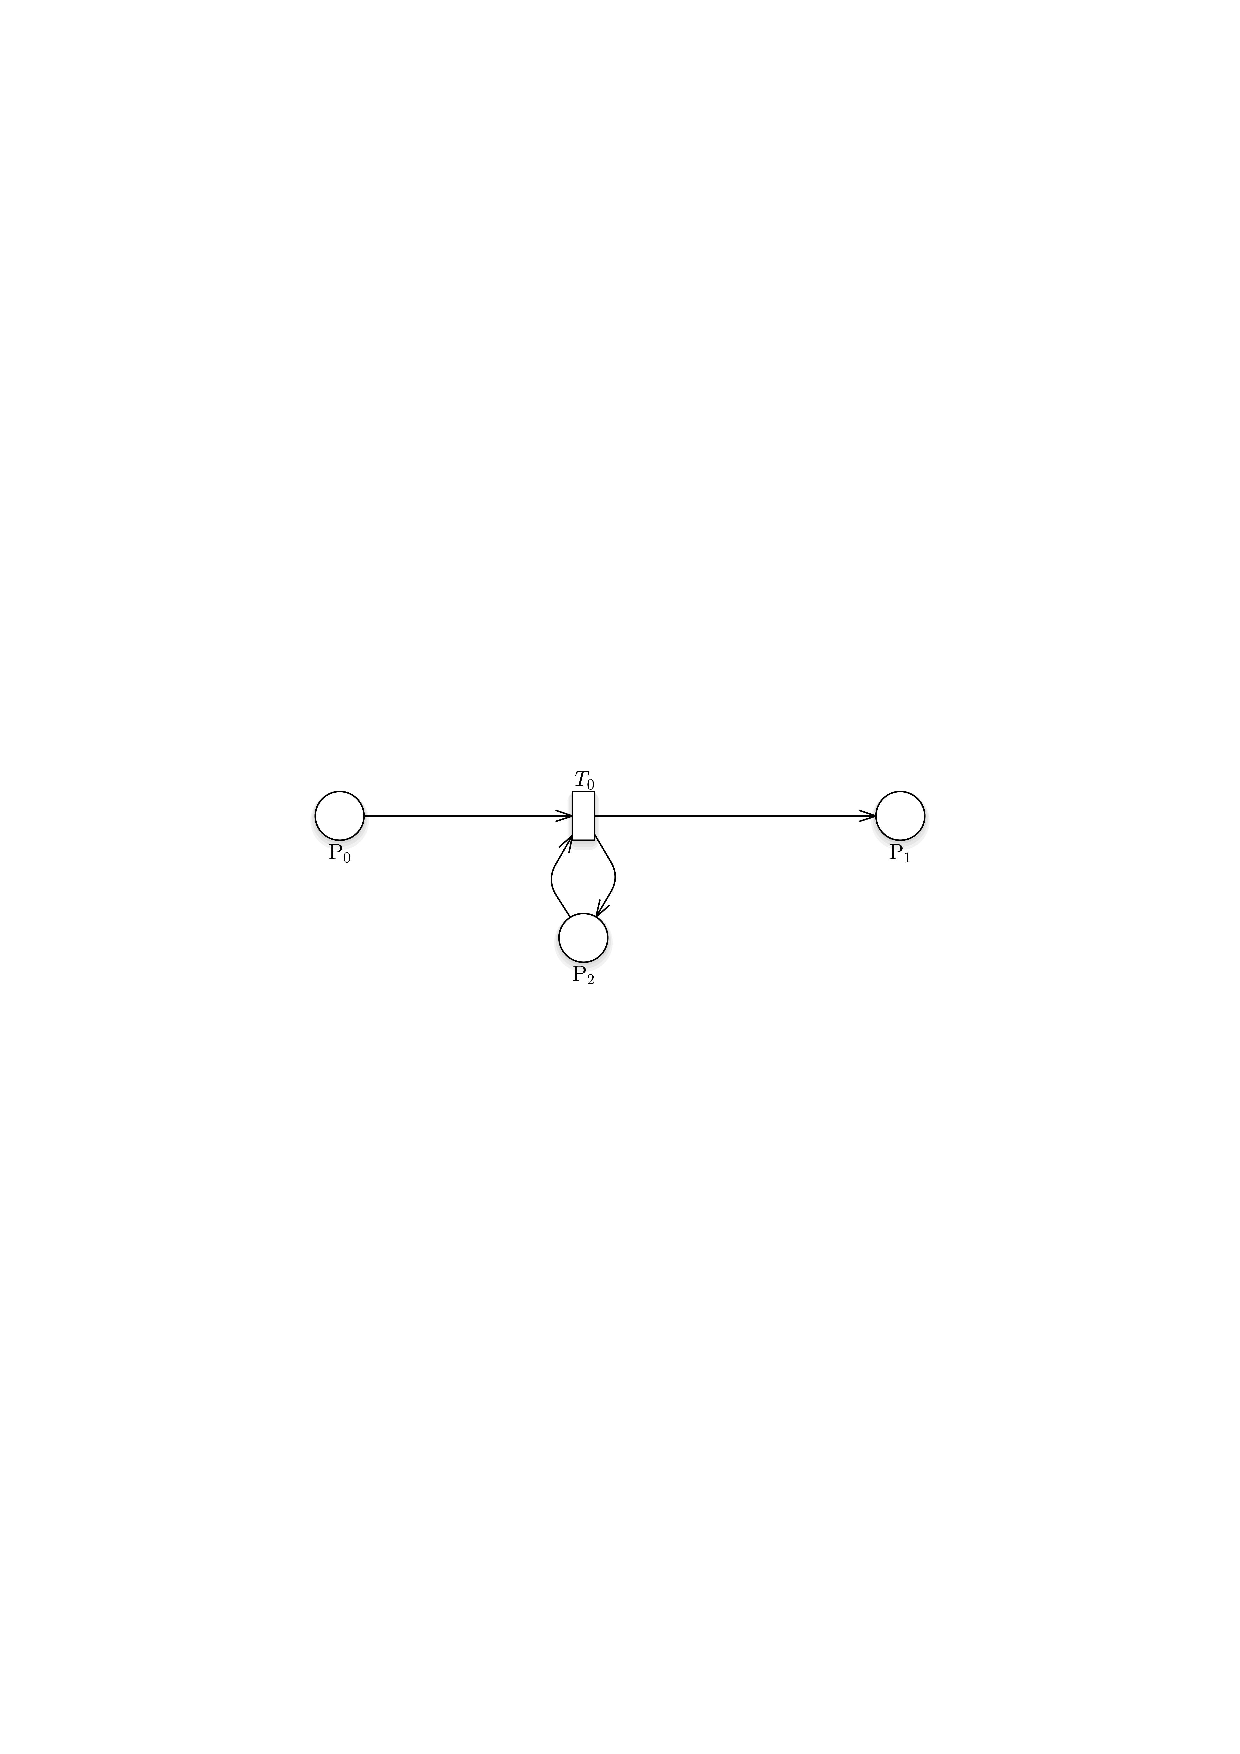
\includegraphics[width=\textwidth]{images/test}
\end{center}
The dataset used in this project was the Enron Email Dataset, provided at \cite{dataset}. This dataset is said to contain over 500,000 emails from 150 employees of Enron, with the majority of emails are timestamped between August 1999 and May 2002.
\newline

In all our jobs we processed dataset in its raw format, without doing any cleaning beforehand. The reasoning behind this is that we wanted each individual job to be able to handle a different dataset without any preprocessing having to be run first.
In the development of the jobs we used a subset of the dataset which only contained the first 500,000 lines, and was thereby able to speed up testing. In comparison the full dataset contains 33,834,245 lines of text.
\newline

However, if the dataset were much larger it would not be feasible to clean it up for every job, and we would have to clean it up beforehand. A general cleanup strategy suitable for this particular dataset would be to first properly identify where a message begins and ends, then to remove duplicate messages, and lastly to remove messages missing \verb!From:! and \verb!To:! header fields. Note that is only required when processing the dataset line-by-line, and not when using Hive.
\newline

As several messages contain the entire header of previous sent messages in the body text, it is not sufficient to simply check for the \verb!Message-ID! text to identify the beginning of a new message. A better strategy is to check if the folder the message is sent from is contained on the same line as \verb!"Message-ID:!.
\newline
To remove duplicates we could, similarly to what is done in our jobs, generate a checksum of each entire message, and match if against others. The input data to the hashing algorithm should exclude the first line of the message containing \verb!Message-ID:!, and the one containing \verb!X-Folder:!. The remaining header-fields should be turned into lowercase, as some header-fields may capitalised in duplicates. The full body text can be added as input data. 
\newline

Since some messages don't contain a valid email-address, but and rather a text representation of the sender or recipient, it is quite difficult to map these up to the correct email-address. A solution to this would be the one deployed in several of our jobs, which is to simply exclude all messages which neither contain a valid \verb!From:! or \verb!To:! header field. This can be achieved by adding a simple regex filter. Note that in some cases this condition would be too strict, as one might be more interested in the actual content of the message rather than who sent or received it.


\section{Hadoop setup}
\label{sec:hadoop}
To run Hadoop on our local machines we have, in addition to the local setup, created a virtual cluster inside three Docker containers. This is an enhancement to the setup created in lab 4. Instructions and files can be found at \url{https://gitlab.com/mindejulian/docker-hadoop-cluster}.
\subsection{Docker setup}
\label{sec:docker}
The Dockerfile contains, and will upon build execute all commands needed to create the Hadoop cluster base image from a clean and minimal Cent OS image. To start a cluster of one namenode and two datanodes we use the \verb!start-cluster.sh! script, which first sets up a local bridge network for the containers to live on, and then starts up the master node and the two slaves.
\begin{verbatim}
sudo docker run -itd \
                --net=hdp-cent \
                -p 50070:50070 \
                -p 8088:8088 \
                -p 19888:19888 \
                -v $(pwd)/../etcs/dis_materials:/dis_materials \
                -v $(pwd)/configs:/usr/local/hadoop/etc/hadoop \
                -v $(pwd)/data-master:/hdfs/data \
                -v $(pwd)/../emails.csv:/emails/emails.csv \
                -v $(pwd)/metastore_db:/metastore_db \
                --name hadoop-master \
                --hostname hadoopmaster \
                --ip 10.0.1.200 \
                --add-host=hadoop1:10.0.1.201 \
                --add-host=hadoop2:10.0.1.202 \
                mindejulian/hdpcent
\end{verbatim}
Here we use Dockers \verb!run! command and set the flags \verb!i!, \verb!t! and \verb!d! right away. \verb!i! for interactive mode, so it will not shut down when it's done executing whatever it starts with. \verb!t! tells Docker to allocate a tty connection and log us in to it locally, and \verb!d! makes it run in the background (detached), so it will stay on even if we close our tty session. Then we need to connect some ports of the container. \verb! -p 50070:50070! maps port 50070 on the container to \verb!localhost:50070! so we can visit the hdfs web interface from our browser. Same goes for \verb!8088! for jobscheduler and \verb!19888! for jobhistory.
\newline
Next we mount the volumes using the \verb!-v! flag; it takes two arguments separated by \verb!:! so \verb!-v $(pwd)/../etcs/dis_materials:/dis_materials ! will mount the folder \verb!$(pwd)/../etcs/dis_materials! as \verb!/dis_materials! on the master nodes file system. If there is already something there, like in the case of the config files, Docker will keep the files and overlay that path with whatever you mount, so the original config files are there but temporarily overwritten by the volume mounted on top. So we mount first the \verb!dis_materials! folder, then the config files for Hadoop, and hive in the same folder. Next we mount an initially empty folder to the path \verb!/hdfs/data!, this is the folder hdfs will use to store data, so by mounting it we do not have to reformat our hdfs everytime we boot the container. Next we mount the emails.csv file and then the \verb!metastore_db! folder for hive to keep its derby server, this also to keep settings between boots.
\newline
The node gets a name, a hostname and an ip, through self explanatory arguments. We then add the other hosts to the \verb!/etc/hosts! of the container. The host file of the container are among others administered by Docker. We tried to add hosts to it in installation, but Docker overwrites them, so to get them in you need to add them like this it seems. Finally we tell what image to use, in this case it should match the name used when building the Docker image from file. \cite{dockerdocs}
\newline
Some of the simpler jobs ran perfectly fine on the default configuration, but as the jobs got bigger we had to increase the heap size to \verb!2048! for map operations and \verb!4096! for reduce operations in  \verb!mapred-site.xml!
\begin{verbatim}
<property>
    <name>mapreduce.map.memory.mb</name>
    <value>2048</value>
</property>
<property>
    <name>mapreduce.reduce.memory.mb</name>
    <value>4096</value>
</property>
\end{verbatim}
This setup work very nice and does not feel as heavy as running three virtual machines, its fast and responsive even on a laptop machine. It does however live on top of a dynamic resource allocation, so the running times gathered from this cluster setup might not be completely representative.
\subsection{AWS}
Amazon web services came through, and gave us \$150 to play with on their services, and we are very impressed with how seamlessly it integrates with MRJob.
\newline
The setup is super simple, as long as you don't try to be a smart ass and say you want to use the datacenter in Frankfurt, that did not work. I think it was because of some verification and signing issues, but did not investigate it as it was simpler to move to the default Oregon datacenter.
\newline
Running jobs on AWS EMR seems to take forever compared to running locally, and it is probably caused by the setup bias. It takes time to start up EC2 instances and move data around, it even says it waits 10min for the logs to be transferred to S3 after it is done, so its obviously made to run bigger things than our one step jobs on a relatively small dataset. It seems very fast when it gets going though, and the difference between running on a 10k lines subset and the full set is smaller than expected, as we will see in some of the job descriptions below. Configuring the EMR runner was very simple as well, and we used a very standard config, except for one job where we used 4 instances of the more powerful \verb!m3.2xlarge! machine.
\section{Key Map Reduce algorithms implemented}
\label{sec:mapreducealgorithms}
% Counting emails
\subsection{Counting emails}
\label{sec:41_counting}
In order to get familiar with the dataset we wanted to know how many emails it contains, and how many of them are unique. We have two approaches to this problem.
\subsubsection{Counting Message-IDs} 
\verb!MRGetMessageId! consists of one mapper and two reducers. The first mapper, \verb!mapper_count! checks if the line contains a message id. If there is a valid message id, it will yield this, if not it will do nothing; if it sees \verb!Message-ID:! but cannot find an id between two brackets ($<$ and $>$) it will yield 1 to \verb!no_id_found!. 

\begin{verbatim}
@staticmethod
def get_msg_id_from_line(line):
    """
    This method takes a line and returns the message id if
    one is found. no_id_found is returned if the keyword
    Message-ID is found but not a properly formatted id.
    The regexp returns anything between < and >. If the
    keyword is not found, keyword_not_found is returned.
    """
    line = line.strip()
    # If Message-ID is part of the line, its the
    # first line in a message.
    if line.find('"Message-ID:') != -1:
        # extract the Message-ID
        match = re.match(r"^.*<(.*)>.*$",
                         line[line.find('"Message-ID'):])
        if match:
            message_id = match.group(1)
            return message_id
        else:
            # If the message id is not found return no_id_found
            return 'no_id_found'
    else:
        return 'keyword_not_found'
\end{verbatim}
The first reducer checks if the key is \verb!no_id_found! it yields the same key but with the sum of values, if the key is different, meaning it is a unique message id, it yields \verb!unique_msg_id! with a 1, and \verb!total_msg_ids! together with the sum of the values.

\begin{verbatim}
        def reducer_count(self, key, values):
        if key == 'no_id_found':
            yield key, sum(values)
        else:
            yield 'unique_msg_id', 1
            yield 'total_msg_ids', sum(values)
\end{verbatim}

This second reducer, sums up the values and yields the result. 
\newline
Running this on the full dataset gives
\begin{verbatim}
"Total number of Message-IDs"        517401
"Unique Message-IDs found"           517401
\end{verbatim}
% TODO Running times locally and EMR
So we have a total of $517401$ emails, and all of them have unique message ids.
\newline
Running this very small and simple job locally using \verb!MRJobInlineRunner! it took $166$seconds or $2$min$46$seconds. This is not an exact measurement as it is highly dependent on available cpu and memory on the computer it runs on, but it does give an indication.
\newline 
Running the same job on the docker cluster which is running on top of the same machine and thus have less resources, took $2$min $6.483$ seconds. In this scenario the input files were already added to hdfs. But still it seems to actually be faster to run this job on Hadoop with all the overhead created by docker than running it inline locally. 
\newline
Running this job on AWS EMR is not comparable in this case, if we just look at the time spent doing map and reduce tasks and don't count the time to setup cluster and move data it still ends up using $108.5 + 160.4 = 268.9$ seconds or $4$min $29$seconds. We assume this happens because the steps are so simple, and thus distributing it over many instances costs more than we gain.
\begin{verbatim}
...
Total time spent by all map tasks (ms)=36181
Total time spent by all maps in occupied slots (ms)=108543
Total time spent by all reduce tasks (ms)=40095
Total time spent by all reduces in occupied slots (ms)=160380
...
\end{verbatim}
\subsubsection{Hash the content and compare.}
The results from \verb!MRGetMessageId! were ok, but they seemed too perfect, so we kept at it, trying to find something wrong with our interpretation of the emails.
\newline
We studied the dataset some more and found that there were some emails that looked exactly the same when comparing time, addresses, subject and body, but leaving out the \verb!Message-ID!. To weed out these duplicates we took the whole emails, headers and all, everything between two message ids really and make a hash of it. We did this in the \verb!MRCountDuplicateEmails! job. And it gave the same results as above. So we modified \verb!MRCountDuplicateEmails! to ignore both the \verb!Message-ID! line and the \verb!X-Folder! line, also the rest of the header fields were made lower case, and then the results were very different.

\begin{verbatim}
def mapper_count(self, _, line):
    """
    Reads a complete email, with headers and all, and make a hash
    of this.
    Yields the hash as key and 1 as value.
    """
    # If Message-ID is part of the line, its the first line in
    # an email.
    if line.find('"Message-ID:') != -1:
        if self.in_msg:
            # we need to finish the last email first. Since this
            # is the beginning of the next.
            if len(self.text) > 0:
                chk = hashlib.md5(self.text).hexdigest()
                yield chk, 1
            self.text = ''
        self.in_msg = True
    # ignoring the message id line
    elif self.in_msg:
        # If we are in the message, append the line and move on,
        # unless its the X-Folder line.
        if line.find('X-Folder:') != 0:
            self.text += line
\end{verbatim}
The output after running this on the full dataset
\begin{verbatim}
"Total number of emails"        517399
"Total number of unique emails" 292728 
\end{verbatim}
By the modified hash method we get a total of $517399$ emails and $292728$ of them are unique. Consequently $224671$ or $43\%$ of the emails are duplicates. As this is a considerable amount of duplicates, in some of the jobs you will see in this report we have worked with the duplicate free set, in some we have an option for it, and in some of them we only work with the original set.
% Running times
\newline
This job has few steps, but collecting the full email and hashing are time consuming operations. The inline running time is $2$minutes and $54.661$seconds. Running this job in the docker cluster took $2$minutes $19.986$seconds.
\newline
% Identifying email threads.
\subsection{Identifying email threads}
\label{sec:emailthreads}
Emails often get forwarded and replied to, sometimes the first email is part of the body of the reply, but it seems these parts have been removed in this dataset. Removing them makes the analysis of the emails in general a lot easier, but finding threads a lot harder. The emails in a thread do not have to share any attributes, there is no way to truly identify a thread by the emails headers, nor the text or subject, so however this is done there will be room for error. However we wanted to try to connect emails in a thread based on the subject line. Very often people do not change this when replying to, or forwarding an email. Another thing emails in a thread must have in common are the email addresses. So if the subject is the same and the email addresses match, they are part of the same thread.
\newline
The job \verb!MREmailThreads! consists of two steps, the first having a \verb!mapper_init!, a \verb!mapper! and a \verb!reducer!, while the last step only has a \verb!reducer!. A static class variable \verb!IGNORE_DUPLICATES! determines if the job should ignore the duplicates found in \verb!MRCheckForDuplicates! or use the full set.
\\
The first mapper parses the emails and cleans the subject, removing all \verb!Fw:! and \verb!Re:! and such.
\\
If we run with \verb!IGNORE_DUPLICATES! this first mapper uses the hash as key, and email object as value. We then run an extra reducer \verb!reducer_dupes! that yields the first email in values, with its subject as key.
\newline
The \verb!reducer_email!s job then is to connect the emails that have the same subject and same addresses, and yield a thread dictionary.
\begin{verbatim}
def reducer_email(self, subject, emails):
    """
    Connect emails that have same subject and some of the 
    same people into a thread.
    :param subject: Subject of email, stripped of Re and Fw
    :param emails: Generator that outputs emails from last step
    :return: dictionary containing all info about the thread
    """
    if subject in self.STOP_SUBJECTS:
        yield 'stopped_subject', subject
    else:
        thread = {}
        all_involved = []
        thread['number_of_emails'] = 0
        for email in emails:
             if 'from' in email.keys() and 'to' in email.keys() \
                        and 'subject' in email.keys():
                if len(all_involved) == 0:
                    # First case
                    all_involved.append(email['from'])
                    all_involved.append(email['to'])
                    thread['number_of_emails'] += 1
                else:
                    if email['from'] in all_involved:
                        # If the sender has been involved in this thread before,
                        # include all addresses he added to the thread.
                        thread['number_of_emails'] += 1
                        if isinstance(email['to'], list):
                            for to in email['to']:
                                if to not in all_involved:
                                    all_involved.append(to)
                        else:
                            # email['to'] must be a string
                            if email['to'] not in all_involved:
                                all_involved.append(email['to'])

        thread['involved'] = all_involved
        thread['subject'] = subject

        if thread['number_of_emails'] > 1:
            yield 'threads', thread

\end{verbatim}
The first thing this reducer does is to check if the subject is in the class list \verb!STOP_SUBJECTS!. This is a list containing subjects that we do not want counted, like empty subject and mailbox full warnings. If the subject is in the stop list, the reducer will yield the subject with the key \verb!stopped_subject!. If the subject is not in this list, the reducer sets up a dictionary \verb!threads!, and a list \verb!all_involved!. 
\newline
Then it iterates over all the emails that share a subject, and checks that they all have the keys needed. If there was something wrong with some formatting or something that caused some keys not to be set, we ignore it and continue. If this is the first, we add both sender addresses and receiver addresses to the all involved set, and increase \verb!thread['number_of_emails']! by $1$. If this is not the first we will add only the recipients, and only if they are not already in the list. We then put the working variables on the \verb!thread! object and yield it if there is more than 1 email, if there is only 1 email in the thread it is not really a thread. 
\newline
The last reducer sums up and yields the results.

\begin{verbatim}
Thread ignored: : HourAhead Failure <CODESITE>
Thread ignored: : WARNING:  Your mailbox is approaching the size limit
Total number of emails in threads: 261414.0
Minimal number of emails in one thread: 2.0
Subject of the minimal email: TransPecos LOI
Maximum number of emails in a thread: 338.0
Subject of the maximal email: Williams Energy News Live -- today's video newscast
Average number of emails in a thread: 3.79
Total number of addresses involved in threads: 146286.0
Minimal number of emails in one thread: 2.0
Subject of the minimal email: (01-123) NYMEX BOARD EXTENDS PROPRIETARY FEE REDUCTION PROGRAM
Maximum number of addresses involved in a thread: 33.0
Subject of the maximal email: Access to UBSWenergy Production Environment
Average number of addresses involved in a thread: 2.12
\end{verbatim}
When the reducer gets the key \verb!stopped_subject!, it yields \verb!Thread ignored: ! with the subject as value.
\newline
To run this job you can use the usual procedure by calling the class directly, or you can use the \verb!email_therads_runner! which will collect the results and draw a scatterplot.
\verb!all_emails! is the number of emails for each of the threads, while \verb!all_involved! is the number of addresses involved in each thread.
\newline
Fig. 1 shows the scatterplot after running on the whole dataset without duplicates. As expected most threads are located in the lower left corner, low number of people involved, and not many emails sent. And the line forming along the bottom line shows that there are alot of emails that go out to alot of people but get little response, I think we can all recognise this concept. What is interesting is the left side of the plot. There is a line forming along the $y$ axis, but it seems to bend inwards. It seems that there is an upper limit to emails with few people and the more people in the conversation the more emails can go back and forth. Are there no small groups of people that keep a thread alive for ages here? Or maybe these are emails that go out to a group of people and the majority responds.
\begin{figure}[h]
	\begin{center}
		\includegraphics[width=\textwidth]{images/to3}
	\end{center}
	\caption{Emails vs participants, without duplicates}
\end{figure}
Running this job on the full set on the Docker cluster took 3minutes 12seconds, while on AWS EMR using the default setup it took 44minutes 36seconds. We suspect this is a fluke, the difference cannot be that big, and we have not seen such big differences in any of the other jobs we have compared.
% TODO Running times locally and EMR 
% Runningtime on Docker cluster 3m12.076s
% Total runningtime on AWS EMR 44m36.594s

% Send times % 
\subsection{Send times}
\label{sec:sendtimes}
With this job we wanted to see at what time of day, and which day of the week people send emails.
\newline
The job \verb!MRSendTime! has one mapper and one reducer. The \verb!mapper! finds the line that starts with \verb!Date:! and then tries to parse the rest of that line into a python datetime object. It then yields a 1 with a tuple containing the number of the weekday and the hour the email was sent as key. If it cannot parse the date we ignore it. Our results suggest that this happens to very few emails, and it is reasonable to belive that the dates of such emails have the same distribution as the rest of the set, thus loosing a few times is not a problem for our goal.

\begin{verbatim}
if line.find('Date: ') == 0:
    try:
        date = parse(line[6:])
        yield (date.weekday(), date.hour), 1
    except ValueError:
        pass
\end{verbatim}
The reducer now gets one hour of the week at a time, and yields one dictionary with keys \verb!weekday!, \verb!hour! and \verb!amount!.  
\begin{verbatim}
weekday = key[0]
hour = key[1]
yield key, {'weekday': weekday, 'hour': hour, 'amount': sum(values)}
\end{verbatim}
This job is best run with a runner that can visualise the output as seen in Fig. 2.

\begin{figure}[h]
	\begin{center}
		\includegraphics[width=\textwidth]{images/sendtimes}
	\end{center}
	\caption{Email send time for each day of the week}
\end{figure}
% TODO Running times locally and EMR
To run this job with the inline runner took $4$minutes $19.514$seconds, while running it on EMR took $30$minutes $39.386$seconds in total from start to stop. If we count just the time spent by map and reduce tasks EMR took $18$minutes $21$seconds to finish.
\begin{verbatim}
Total time spent by all map tasks (ms)=942724
Total time spent by all maps in occupied slots (ms)=2828172
Total time spent by all reduce tasks (ms)=17420
Total time spent by all reduces in occupied slots (ms)=69680
\end{verbatim}
\subsection{Identifying internal community structures}
\label{sec:comstruct}
This job focuses on identifying which persons are most likely to have meaningful collaboration, and uses this information to draw a graph of an internal community structure. The structure is a set of groups, where each person within is classified to have a large part of their communication within the group. Each person is placed in only one group.
\newline
\newline
For communication between two parties to be quantified as meaningful by our algorithm, we introduce a parameter called \verb!Weight!. Weight between two parties is accumulated for every message exchanged, where the weight for each message is total number of characters in the text divided by number of receivers. We require that both parties have sent at least 15 email-messages to each other. Further we require that the weight between the two parties is at least 9000 in both directions, and at least 21000 in one direction. In addition we allow clusters to merge if two people in different clusters have a weight of at least 54000. To achieve a weight of 21000 over a two-year period one could for example send 70 emails to only the recipient with each message containing 300 characters. Note that this is roughly one and a half email a month over a two year period. The values for the requirements are easily configurable through the command line options \verb!--minRelWeight!, default 21000, \verb!--minNbWeight!, default 54000, \verb!--minCorrespondanceWeight!, default 9000 and \verb!--minCorrespondance!, default 15.
\newline
\newline
To filter out sender and recipients, this job bases itself on the discussion about duplicates in section~\ref{sec:2_dataset}. However, this job also requires both the \verb!From!, and \verb!To!, to be filled with valid email addresses, where only addresses with postfix @enron.com are counted. In addition we have identified four addresses which do not belong to any one person, and are therefore excluded from the community structure. These are: 'no.address@enron.com', 'enron.announcements@enron.com', 'announcements.enron@enron.com', 'outlook.team@enron.com'. Lastly, we noticed that users have different \verb!From:! fields in their \verb!sent_items! folders. For example Phillip Allen has sent messages with both phillip.allen@enron.com and k..allen@enron.com. We purposely did not merge these, as we cannot be sure about whether people actually communicated using several addresses, or the data quality is low in this regard.
\newline
\newline
To implement this job we developed a 3-step MapReduce algorithm. The first step of job has a mapper along with an initialiser and a reducer, the second a mapper, a combiner and a reducer, and the last step only has a reducer. The following two images display an overview of the input and output of each phase. After these, each phase will be described in detail.
\begin{center}
		\includegraphics[width=\textwidth]{images/communityStep1}
		\includegraphics[width=\textwidth]{images/communityStep2}
	\end{center}

The first step in the algorithm reduces the amount of emails we have to evaluate. Where the mapper does the filtering part, and the reducer removes the duplicates.
The mapper used in the first step is inspired by the \verb!MRMultilineInput! job given in the course material.
\verb!mapper_email! starts by checking if the line is the first line in a message. This is done with \verb!MRGetMessageId!, which will return \verb!keyword_not_found! if the folder where the email was stored is not on the same line. This means that it will not trigger when a body text contains the string \verb!Message-ID!. If it returns the actual message-id, we know that we are at the beginning of a new email, and we want to yield the one already processed, and reset the mapper variables.
Once we reset mapper variables and start processing the email message, we concatenate lower case of all header fields except the ones containing \verb!X-Folder! and \verb!Message-ID! into a variable \verb!emailHashLines!. The header field $From$ is ran through the function \verb!get_email_from_line! which contains a regex filter and will yield $None$ if the line does not contain a valid email address with postfix @enron.com. If the regex filter finds a match the email is added to \verb!email['from']!. The \verb!To! header file is added directly to \verb!email['to']!.
\newline
\newline
Once we hit the header field \verb!X-FileName! we know that the following line will be part of the body text, and therefore set a local variable \verb!in_body! to $True$.
When we are in the body text we concatenate all lines into \verb!emailHashLines!, and we add up the length of each line into \verb!email['body_count']!. 
\newline
\newline
A value is only yielded if both $to$ and $from$ are added to the \verb!email! dictionary. The $from$ address must also be different to the set of email-addresses which we have chosen to ignore from the community structure.
The key-value pair yielded is a MD5 checksum of the variable \verb!emailHashLines! as the key, and the dictionary \verb!email! as value.


\begin{verbatim}

    @staticmethod
    def get_email_from_line(line, onlyEnron=None):
        if onlyEnron:
            match = re.search(r'[\w\.-]+@enron.com', line.lower())
        else:
            match = re.search(r'[\w\.-]+@[\w\.-]+', line.lower())
        if(match != None):
            return match.group(0)
        return None
        
        
    def mapper_email(self, key, line):
        line = line.strip()
        # If Message-ID is part of the line, its the first line in a message.
        msgId = MRGetMessageId.get_msg_id_from_line(line)
        if msgId != 'no_id_found' and msgId != 'keyword_not_found':
            if self.in_email:
                if 'from' in self.email and 'to' in self.email and \
                                self.email['from'] not in self.IGNORE_EMAILS:
                    chk = hashlib.md5(self.emailHashLines).hexdigest()
                    yield chk, self.email
                self.in_email = False
                self.in_body = False
                self.emailHashLines = ''
                self.email = {'body_count': 0}
            self.in_email = True

        if self.in_email:
            if line.find('X-Folder:') != 0 and not self.in_body and \
                    (msgId == 'keyword_not_found' or msgId == 'no_id_found'):
                # Lowercase all metadata for better detection of duplicates.
                self.emailHashLines += line.lower()
            if self.in_body:
                self.emailHashLines += line
                self.email['body_count'] += len(line)
            # X-FileName indicates that the next line is the first in the body
            elif line.find('X-FileName') == 0:
                self.in_body = True
            else:
                if line.find('From:') == 0:
                    rawFromAddr = line[5:].strip()
                    fromAddr = self.get_email_from_line(rawFromAddr,True)
                    if fromAddr is not None:
                        self.email['from'] = fromAddr
                if line.find('To:') == 0:
                    self.email['to'] = line[3:].strip()
\end{verbatim}

The reducer implementation is quite simple, as we only want to yield unique email messages. Therefore we yield the first item in the list of emails which has the same MD5 hash.

\begin{verbatim}
    def reducer_email(self, key, value):
        l = list(value)
        yield None, l[0]
\end{verbatim}

In the second step our goal is to aggregate the results of step one, and to filter out data that does not meet our requirements. To do this we first have the mapper calculate the weight for each message sent. Then the \verb!To:! metadata field is split into individual addresses. Each of these addresses are then filtered with check if they have the postfix $@enron.com$ and belong to a single person. If found true, the key-value pair is yielded with $(From, To)$ as the key, and $(weight, 1)$ as the value. Note that 1 here means the count.

\begin{verbatim}
    def mapper_from_to(self, key, email):
        if 'to' in email.keys() and 'from' in email.keys() and 'body_count' in email.keys():
            to = email['to'].split(',')
            weight = float(email['body_count']) / float(len(to))
            for to_addr in to:
                rawToAddr = to_addr.strip()
                toAddr = self.get_email_from_line(rawToAddr,True)
                # Only yield valid, non-ignored emails not equal to sender.
                if toAddr is not None and toAddr not in self.IGNORE_EMAILS and \
                                email['from'] != toAddr:
                    yield (email['from'], toAddr), (weight, 1)
\end{verbatim}

After the mapper phase follows the combiner and then the reducer. The job of the combiner is to reduce the amount of data being sent to the reducer. This is achieved by aggregating the results of the mapper for each $(From, To)$ pair. The reducer also aggregates the results it receives, but only yields if both \verb!Count! \verb!Weight! is above our defined thresholds. In addition we want the next step to only have one instance of a reducer, and there set the yielded key to $None$, and the value to a tuple on the form $(From, To, Weight, Count)$.

\begin{verbatim}
    def combiner_from_to(self, key, values):
        z = zip(*list(values))
        yield key, (sum(z[0]), sum(z[1]))

    def reducer_from_to(self, key, values):
        z = zip(*list(values))
        count = sum(z[1])
        weight = sum(z[0])
        if float(weight) >= self.options.minCorrespondanceWeight \
                and float(count) >= self.options.minCorrespondance:
            yield None, (key[0], key[1], weight, count)
\end{verbatim}

In our last step we only have a single reducer. Since we did not want a person to be member of more than one cluster, we opted to only run a single instance of the reducer. 
\newline
In this phase we start by sorting the values by weight in ascending order. Then we start to iterate through the sorted list, we first search the local dictionary \verb!communicationNodes! if the reverse pair $(To, From)$ exists. If it does, we know that communication in both directions fulfils our requirements, and that $(From, To)$ pair is the stronger of the two. If the pair does not exist, we simply add it to the dictionary and continue to the next item in the list.
\newline
Once we know that strong enough communication exists in both direction we start processing the $(From, To)$ pair. First we check if the two nodes already exist in the same cluster, and if so we can simply continue to the next item in the list. If they do not, we start checking if either node is already connected to a cluster. We do this by checking the dictionaries \verb!clusterNodes! and \verb!nodeToCluster!. \verb!clusterNodes! contains an entry for every cluster, where the root node is the key, and a list of node contained in the cluster as value. It is constantly manipulated for every item iterated, and is finally yielded at the end of the reducer. \verb!nodeToCluster! is a dictionary which has a node as the key, and which cluster it belongs to as value. It is used for easy lookup when we need to know if we already added a node a cluster, and also where it is located.
\newline
Once we know if either node in the $(From, To)$ pair already exists in a cluster we will add the other node to the same cluster. This is conditioned by a weight of at least 21000 between them, and that the pair does not exist in another cluster already. If both nodes already exists in different clusters, we will merge the two clusters if the weight is at least 54000. If neither node is added to a cluster, a new one will be created.
\newline
\begin{verbatim}
def reducer_community(self, key, value):
    clusterNodes = {}
    nodeToCluser = {}
    communicatingNodes = {}
    # Sorts so that lowest weight edge is iterated first.
    sorted_List = sorted(list(value), key=lambda sec: +sec[2])
    for elm in sorted_List:
        if ((elm[1], elm[0]) in communicatingNodes.keys()):
            # Sorted by weight. Know that the reverse edge has the same or higher weight.

            # Nodes are already in the same cluster. Continue.
            if (elm[0] in nodeToCluser and elm[1] in nodeToCluser and \
                    nodeToCluser[elm[0]] == nodeToCluser[elm[1]]) or (elm[0] in \
                    nodeToCluser and nodeToCluser[elm[0]] == elm[1]) or (elm[1] \
                    in nodeToCluser and nodeToCluser[elm[1]] == elm[0]):
                continue

            if float(elm[2]) >= self.options.minRelWeight:
                # Check if second node already has a cluster of his own.
                if elm[1] in clusterNodes:
                    ..............

                # Check if second node is already added to another cluster.
                # Merge contents into the largest clusters, if first is also in another
                # cluster.
                elif elm[1] in nodeToCluser:
                    if elm[0] in nodeToCluser:
                        if float(elm[2]) >= self.options.minNbWeight:
                            ..............

                    # First node is a startNode. Check the length of it before merging.
                    elif elm[0] in clusterNodes:
                        ..............

                    # Does not exits a start node for first yet. Simply add it to seconds
                    # cluster
                    else:
                        clusterNodes[nodeToCluser[elm[1]]].append(elm[0])
                        nodeToCluser[elm[0]] = nodeToCluser[elm[1]]

                    continue

                # Check if first node is already in another cluster. If so,
                # add second to it.
                elif elm[0] in nodeToCluser:
                    ..............

                # If first node does not have a cluster. Create one.
                elif(elm[0] not in clusterNodes):
                    clusterNodes[elm[0]] = list()


                clusterNodes[elm[0]].append(elm[1])
                nodeToCluser[elm[1]] = elm[0]

        else:
            communicatingNodes[(elm[0], elm[1])] = {'weight': elm[2], 'count': elm[3]}

    for node in clusterNodes:
        yield node, clusterNodes[node]

\end{verbatim}

The final output will have the root node as the key, and a list nodes contained in the cluster as value. Similar to the following:
\begin{verbatim}
"chris.germany@enron.com"	["joan.veselack@enron.com", "joann.collins@enron.com", ........]
"ed.mcmichael@enron.com", "ruth.concannon@enron.com", "victor.lamadrid@enron.com", ........]
"megan.parker@enron.com"	["j..farmer@enron.com"]
"virginia.thompson@enron.com"	["bill.williams@enron.com", "cara.semperger@enron.com", ........]
"andrew.edison@enron.com"	["b..sanders@enron.com", "gail.brownfeld@enron.com"]
"monika.causholli@enron.com"	["e..carter@enron.com", "david.allan@enron.com"]
"rick.bergsieker@enron.com"	["mike.mcconnell@enron.com", "cathy.phillips@enron.com", ........]
"trevor.woods@enron.com"	["e.taylor@enron.com"]
"rob.walls@enron.com"	["james.derrick@enron.com", "j.harris@enron.com"]
"alexandra.villarreal@enron.com"	["john.griffith@enron.com"]
"mary.poorman@enron.com"	["daren.farmer@enron.com", "julie.meyers@enron.com", ........]
"mark.whitt@enron.com"	["dave.fuller@enron.com", "barry.tycholiz@enron.com", ........]
"phil.demoes@enron.com"	["dan.hyvl@enron.com", "kim.ward@enron.com", "stacy.dickson@enron.com", ........]
"m..presto@enron.com"	["billy.braddock@enron.com", "john.suarez@enron.com", ........]
"barton.clark@enron.com"	["kay.mann@enron.com", "scott.healy@enron.com", ........]
"rod.hayslett@enron.com"	["morris.brassfield@enron.com", "danny.mccarty@enron.com", ........]
"eric.bass@enron.com"	["matthew.lenhart@enron.com", "brian.hoskins@enron.com", ........]
"lynn.blair@enron.com"	["raetta.zadow@enron.com", "steve.january@enron.com", ........]
"w..white@enron.com"	["casey.evans@enron.com", "john.postlethwaite@enron.com"]
\end{verbatim}

We then created a runner, \verb!DrawCommunityGraph! which took this output, and by passing it to the library PyGraphviz we were able to visualise the community structure. The colour of each cluster is chosen at random from a set of 40 colours, and therefore some clusters will have the same colour. The distance between each cluster is constant, with 7 clusters in the width. However each individual node is randomly placed within the area of each cluster.
The full community structure with our requirements is presented in the image below. The second image shows of a subset of the community structure for better readability. It is obvious that it would be possible to improve the visual presentation of the graph by for example disabling overlapping of the nodes and removing the @enron.com postfix from each node.

\begin{center}
		\includegraphics[width=\textwidth]{images/communityGraph_scaled}
\end{center}

The next image shows only a subset of the community structure. 

\begin{center}
		\includegraphics[width=\textwidth]{images/comStructZoom}
\end{center}


\subsection{Search emails using tf-ifd method}
\label{sec:tfids}
To search the emails for specific words or phrases is a task that can have many different approaches and solutions. This  \verb!MRTfidfSearch! job uses the tf-idf method. Tf-idf is short for term frequency-inverse document frequency \cite{wikiTFIDF} and is a method of scoring documents that takes into account how important the word is in the document collection as well as in the document.
\newline
Our implementation takes three commandline arguments, \verb!--query! the word or words to search for, \verb!--numResults! how many results to show, will show all relevant if not set, and \verb!--ignoreDupes! that will check for and ignore duplicates if set to yes or any other string, default is \verb!None!.
\newline
The first mapper parses the email and counts the total number of words and number of each query term present in the email body.
\newline 
In the \verb!reducer_idf!, which is the next operation if \verb!--ignoreDupes! is not set, we first calculate the idf for every term
\begin{verbatim}
for t in qt:
    tot_relevant = sum(1 for x in el if x['qts_in_body'][t] > 0)
    if tot_relevant > 0:
        preidf = float(tot_emails) / float(tot_relevant)
        idf[t] = math.log10(preidf)
    else:
        idf[t] = 0.0
\end{verbatim}
Then we set this idf on every email dictionary and yield it with key \verb!None!. The \verb!mapper_tfidf! will then calculate the tf-idf and total score of the email and yield it if total score is bigger than 0. If it is 0 it means none of the query terms were present in the body and thus it is not relevant.
\newline
The \verb!reducer_tfidf! sorts the list based on the total score and yields the message id, the total score, from address and subject. Since the message id is determined unique, it can be used to get the full email, for example using Hive.
% TODO Running times locally and EMR
\subsection{Finding top senders}
\label{sec:topsender}
The goal of this job was to provide a result which makes fetching an arbitrary number of top senders easy. In addition we wanted to have a job where we could easily compare the execution with Hive. Because we wanted to compare execution with Hive, duplicates were not removed in this task. However this could easily be implemented by using the same approach as discussed in section~\ref{sec:comstruct}, \texttt{\nameref{sec:comstruct}}.
\newline
\newline
The \verb!MRTopEmailSender! job uses 2 MapReduce steps, the first one having a mapper, combiner and reducer, and the last only having a reducer. The following image displays an overview of the input and output of each phase. After these each phase will be described in detail.
\begin{center}
		\includegraphics[width=\textwidth]{images/topsenderSteps}
\end{center}

In similar fashion to the first step of other tasks, the mapper processes the input data line by line, and deploys a modified version of the \verb!MRMultilineInput! job provided in the course material \cite{coursematerial}. There is not much to say about this phase which has not been said already. The only special thing is that we yield the from address as key, and the number of recipients as the value.
\newline
The combiner phase simply aggregates the number of recipients by using the \verb!sum! function. The reducer is similar to the combiner, but it instead yields \verb!None! as the key, and a tuple of $(From, Count)$ as value. The change of key-value in the reducer is done in order to make sure only a single instance of reducer is ran in the second step.

\begin{verbatim}
    def combiner_topsender(self, pair, values):
        yield pair, sum(values)

    def reducer_topsender(self, pair, values):
        yield None, (pair, sum(values))

    def reducer_sort(self, key, value):
        sorted_List = sorted(list(value), key=lambda sec: -sec[1])
        for elm in sorted_List:
            yield elm[0], elm[1]
\end{verbatim}

The reducer in the second step is responsible for sorting each sender in descending order based on how many emails they sent. It then yields with the address of the sender as the key, and the number of emails sent as value. The final output will be on the following form:

\begin{verbatim}
"jeff.dasovich@enron.com"	22244
"kay.mann@enron.com"	21630
"vince.kaminski@enron.com"	15230
"chris.germany@enron.com"	14682
"tana.jones@enron.com"	14232
"sara.shackleton@enron.com"	11324
"pete.davis@enron.com"	9150
"enron.announcements@enron.com"	8820
"steven.kean@enron.com"	7700
\end{verbatim}

By having the result in this format, it is easy for a third party to get how many emails a specific person sent. In addition, to get the top 10 senders, it can simply get the 10 first lines of the output.
\newline
\newline
This task was used in order do a performance comparison between MapReduce and Hive.  We did both measurements in the Docker cluster described in section~\ref{sec:docker}.
The MapReduce task was measured to a total running time of $2$ minutes  $43$ seconds. In section~\ref{hivetopsender} we will take a look how we can use Hive to perform the same task.

\subsection{MRBKMeansClustering - clustering email senders based on their subject lines}
\label{sec:bkmeans}
Bisecting K-means clustering is an extension of the K-means clustering that starts with one big cluster and divides it to two clusters, for then to divide the biggest one of those into two and repeat this process until we have the wanted number of clusters, like an opposite hierarchical agglomerative clustering algorithm. \cite{dat630slides}
\newline
In our implementation we run three repetitions or divisions, ending up with four clusters. We have used the cosine distance between the centroid and the users term vectors as distance measure, where the term vector is the sum of all words used in any subject line by the user. If the flag \verb!--ignoreDupes! is set, there will be an extra step after step 1.
\newline
\textbf{Step 1}. The first mapper yields every word in the subject with the sender as key. Then the \verb!reducer_subjects! will sum up and yield one dictionary for every user.
\newline
\verb!yield None, {'username': user, 'terms': t}!.
\newline
\textbf{Step 2}. \verb!reducer_first_centroids! picks two users at random, and then yields everyone of the other users dictionaries with these two under keys \verb!cent_1! and \verb!cent_2!.
\newline
\textbf{Step 3}. In the mapper of this step we measure the distance from the centroids for all the users. The measurement of distance chosen is the cosine similarity of the term vectors. The users are then assigned to the cluster of which the cosine similarity between the user and the centroid is highest, that is they are most similar. The \verb!reducer_first_distance! then yields one dictionary for every cluster, containing the list of users belonging to the cluster along with the cluster number and cluster size.
\newline
\textbf{Step 4}. Here we make a list of the cluster sizes and determine which is the largest cluster, that's the one we're dividing next. So when we find it we pop of two users and set them as centroids 1 and 2, we also append the old centroids to the respective clusters users lists. Then we add all this info  to every user and yield every user with no key.
\newline
\textbf{Step 5}. Here we basically do the same we did in step 3, only if the distance to the first centroid is largest we keep the cluster assignment, otherwise we assign the user to cluster 3.
\begin{verbatim}
if user['largest_cluster'] == user['cluster']:
    dist_c_1 = self.get_cosine_similarity(user['terms'], user['cent_1']['terms'])
    dist_c_2 = self.get_cosine_similarity(user['terms'], user['cent_2']['terms'])
    if dist_c_1 > dist_c_2:
        user['cluster'] = user['cluster']
        user['closest_to_cent'] = user['cent_1']
    else:
        user['cluster'] = 3
        user['closest_to_cent'] = user['cent_2']
yield user['cluster'], user
\end{verbatim}
\textbf{Step 6 and 7}. Are reruns of steps 3 and 4
\newline
Running on the full dataset, with duplicates, looks as follows, but with email addresses belonging to each cluster as well.
\begin{verbatim}
"cluster 1"	size 751
"cluster 2"	size 5690
"cluster 3"	size 308
"cluster 4"	size 18194
\end{verbatim}
As we see there are big variations in the size of the clusters, this difference would decrease if we split it into more clusters.
\newline
% TODO Running times locally and EMR
Running this job inline takes $6$minutes $56$seconds. 
\newline
Running it on Docker cluster took 8minutes 49.047seconds.
\newline
And running this on AWS EMR takes about forever...
\section{HIVE usage}
\label{sec:hive}
Hive is a relational database running on top of Hadoop and HDFS, and by putting your data into Hive it can easily be queried using a query language, HQL, that is very similar to SQL. Hive lets you use the \verb!LOAD DATA! command to load csv files from HDFS directly into a database. It also supports using external scripts for \verb!MAP! and \verb!REDUCE!. Hive also lets you use joins on your data, like in SQL. \cite{oreilly} Hive converts your queries from HQL to actual MapReduce jobs that is then run on Hadoop, so in theory you could get the same results from writing the jobs yourself, but in most cases, Hive is faster, more robust and allows you to spend less time implementing queries.
\subsection{Loading the Enron dataset into Hive}
Loading a csv file into Hive is rather straight forward, first \verb!CREATE TABLE! then \verb!LOAD DATA! and you are good to go. However this dataset has some limitations due to formatting, so before we could load the Enron dataset into Hive we had to do some search and replace on it.
\begin{verbatim}
cat emails.csv |
sed -e 's#"$#XELIOSK#g' |               
# First we replace any occurence of doublequote(") followed by newline ($) with
# a character sequence not used in the dataset, XELIOSK
tr '\n' ' ' |                           
# Then we replace all newline (\n in tr tool) with space
sed -e 's#XELIOSK#\\"\'$'\n#g' |        
# Next we bring back the newlines that was following a doubleqoute
sed -e 's#","#--XYLOPHONICA--#g' |      
# Now we replace all commas between doublequotes with another character
# sequence --XYLOPHONICA--
sed -e 's#,#-#g' |                      
# And then all commas has to go, we replace them here with -
sed -e 's#--XYLOPHONICA--#","#g'        
# And finally we can bring back the doublequotes with comma between them
>> emails_for_hive.csv
\end{verbatim}
After piping the emails through this, it had newlines only between emails, and no commas inside the email, so it was ready for Hive and we could \verb!LOAD DATA! into a table with two columns, \verb!file! and \verb!msg!
\subsection{Creating tables}
Having the messages in Hive as separate rows is nice, but it's hard to query when the whole email is one string, so we tried to separate the emails.
\newline
Hive supports creating tables from select, so we have created a more usable table like this 
\begin{verbatim}
CREATE TABLE rel_emails AS 
  SELECT 
    regexp_extract(msg, '"Message-ID: <(.*?)\\>') AS msg_id, 
    regexp_extract(msg, 'Subject:(.*?)(-|Mime)') AS subject, 
    regexp_extract(msg, 'From:(.*?)To') AS fromaddr, 
    regexp_extract(msg, 'X-FileName:(.*)') AS body 
  FROM emails;
\end{verbatim}
Now we can for example get the body of the email we found in tf-idf search above like this
\begin{verbatim}
SELECT body 
  FROM rel_emails 
  WHERE msg_id 
  LIKE '19273922.1075855691259.JavaMail.evans@thyme';
\end{verbatim}

\subsection{MRTopEmailSender done with Hive}
\label{hivetopsender}
MRTopEmailSender job above gets the one email address that sends the most emails over the set. It is a relatively simple job in MR, but even simpler in Hive.
\begin{verbatim}
SELECT fromaddr, ranking, counted 
  FROM (
    SELECT fromaddr, counted, rank() OVER(ORDER BY counted DESC) AS ranking
      FROM (
        SELECT fromaddr, COUNT(fromaddr) AS counted 
          FROM rel_emails GROUP BY fromaddr) 
      S) 
  R WHERE R.ranking = 1;
\end{verbatim}
Running this query in Hive on the Docker cluster took $1$minute $3.3$seconds. The map reduce job from above took $2$ minutes $43$ seconds, so Hive is approximately $1$ minute $40$ seconds faster on this particular job.
% Running times! Compare Hive running times with running the MR job above. Why is Hive faster/slower?

\section{Summary}
The project was about locating relevant in formation using Hadoop in a dataset of emails. The dataset used was the Enron Email Dataset\cite{dataset} which contains over 500,000 emails. We were free to decide what information to look for, and we came up with 7 different scenarios of fetching relevant information. These scenarios were implemented as MapReduce jobs in Python. At the start of the project we focused on getting to know the dataset, and therefore created jobs of a low complexity level such as \texttt{\nameref{sec:topsender}}. Once we got more comfortable with the dataset and MapReduce we implemented more complex jobs such as \texttt{\nameref{sec:bkmeans}} and \texttt{\nameref{sec:comstruct}}. With the use of the import functionality in python as well as static methods, we were able to re-use code between jobs. This reduced development time, and made it easier to verify the results of each job.
\newline
\newline
It was discovered that the provided dataset contained a large amount of duplicate emails. While some emails were unique, the ones that were duplicated were not uniformly distributed (some emails were duplicated more than others). Because of this, any sort of analysis and information retrieval is at risk of being significantly skewed or just plain erroneous. Therefore significant effort was made into removing duplicate messages, and filtering out some which did not contain valid data. A detailed discussion about the dataset is found in section~\ref{sec:2_dataset}.
\newline
\newline
To compare Hive and MapReduce, we opted to extract the same information in Hive as the MapReduce job \texttt{\nameref{sec:comstruct}}. By doing this we saw that the running time for this particular job was much lower in Hive compared to MapReduce.


% Keeping this for reference for now %
\begin{thebibliography}{7}

\bibitem{wikiTFIDF} Wikipedia article on Tf-idf. \url{https://en.wikipedia.org/wiki/Tf?idf}
\bibitem{oreilly} Tom White, Hadoop: The Definitive Guide, 2015, \emph{ISBN: 978-1-491-90163-2}
\bibitem{dockerdocs} Docker API Docs, \url{https://docs.docker.com}
\bibitem{dat630slides} Slides from DAT630, Krisztian Balog
\bibitem{dataset} Kaggle. The Enron Email Dataset. \url{https://www.kaggle.com/wcukierski/enron-email-dataset}
\bibitem{coursematerial} Data Intensive Systems Compendium, Tomasz Wiktorski et al.
\bibitem{git} Source code of all tasks developed. GitLab \url{https://gitlab.com/mindejulian/projectDAT500/tree/master}

\end{thebibliography}

\end{document}
